\documentclass[
%draft%     uncomment to activate draft mode (see preamble/proofs)
]{scrbook}   

% preamble -- do not rearrange order of \includes
\KOMAoptions{
    fontsize=8pt,              % set default font size
    DIV=calc,
    titlepage=false,
    paper=150mm:220mm,
    twoside=true, 
    twocolumn=false,
    toc=chapterentryfill,       % for dots: chapterentrydotfill
    parskip=false,              % space between paragraphs. "full" gives more space; "false" uses indentation instead
    headings=small,
    bibliography=leveldown,     % turns the Bibliography into a \section rather than a \chapter (so it appears on the same page)
}
\usepackage[
    top=23mm,
    left=20mm,
    height=173mm,
    width=109mm,
    ]{geometry}
    
\setlength{\marginparwidth}{1.25cm} % sets up acceptable margin for \todonotes package (see preamble/packages.tex).
\usepackage[dvipsnames]{xcolor}
\usepackage[hyphens]{url}       % simple URL typesetting
\usepackage[unicode]{hyperref}  % hyperlinks
\usepackage{booktabs}           % professional-quality tables
\usepackage{nicefrac}           % compact symbols for 1/2, etc.
\usepackage{microtype}          % microtypography
\usepackage{lipsum}             % lorem ipsum at the ready
\usepackage{graphicx}           % for figures
\usepackage{footmisc}           % makes symbol footnotes possible
\usepackage{ragged2e}
\usepackage{changepage}         % detect odd/even pages
\usepackage{array}
\usepackage{float}              % get figures etc. to stay where they are with [H]
\usepackage{subfigure}          % \subfigures witin a \begin{figure}
\usepackage{longtable}          % allows for tables that stretch over multiple pages
\setlength{\marginparwidth}{2cm}
\usepackage[textsize=footnotesize]{todonotes} % enables \todo's for editors
\usepackage{etoolbox}           % supplies commands like \AtBeginEnvironment and \atEndEnvironment
\usepackage{ifdraft}            % switches on proofreading options in the draft mode
\usepackage{rotating}           % provides sidewaysfigure environment
\usepackage{media9}             % allows for video in the pdf
\usepackage{fontspec}
\usepackage[dvipsnames]{xcolor}
\usepackage[most]{tcolorbox}
\usepackage{fix-cm}
\usepackage[parfill]{parskip}
\usepackage{minted}
\usepackage{caption}
\usepackage{float}
\usepackage{longtable}
\usepackage{wrapfig}
\usepackage[nottoc,notlof,notlot]{tocbibind} 
\usepackage{tocloft}
\usepackage[L7x, T1]{fontenc}           % use 8-bit T1 fonts
\usepackage[utf8]{inputenc}             % allow utf-8 input
% languages
\usepackage[main=english, lithuanian, latin]{babel}
% special characters
% \DeclareUnicodeCharacter{2D7}{}         % allow ¡ character
% \DeclareUnicodeCharacter{45E}{}         % allow ў character
% \DeclareUnicodeCharacter{2032}{}        % allow ′ character
% \DeclareUnicodeCharacter{22EE}{}        % allow ⋮ character
%\DeclareUnicodeCharacter{010D}{}        % allow č character
% \DeclareUnicodeCharacter{017F}{}        % allow ſ character
\usepackage{textalpha}                  % allows for greek characters in text e.g. \textalpha = α
\usepackage{textcomp}                   % allows \textrightarrow etc.
         
% Palatino font options
\newfontfamily{\heavycolor}{MetropolisBold}
[Extension = .otf]
\newfontfamily{\contentfont}{Inter}
[Extension = .otf]

\addtokomafont{disposition}{\heavy }  % Palatino for titles etc.
\setkomafont{descriptionlabel}{         % font for description lists    
\usekomafont{captionlabel}\content     % Palatino bold
}
\setkomafont{caption}{\footnotesize}    % smaller font size for captions


\usepackage{mathabx}                    % allows for nicer looking \cup, \curvearrowbotright, etc. !!IMPORTANT!! These are math symbols and should be surrounded by $dollar signs$
\usepackage[normalem]{ulem}                       % allows for strikethrough with \sout etc.
\newcommand{\sdot}{\color{RubineRed}.}
\definecolor{dgrey}{RGB}{76, 76, 76}
\newcommand{\content}{\contentfont \color{dgrey}}
\newcommand{\heavy}{\heavycolor \color{Black}}
\newcommand{\heavyred}{\heavycolor \color {RubineRed}

\makeatletter
\newcommand\HUGE{\@setfontsize\Huge{50}{60}}
\makeatother    
}

\captionsetup[figure]{labelfont={bf},name={\heavy Figure},labelsep=period}
% No (sub)sections in TOC
\setcounter{tocdepth}{0}                

% \renewcommand*\contentsname{Contents\sdot}
\addto\captionsenglish{
    \renewcommand*\contentsname{\huge\heavy Contents\sdot}
    \renewcommand{\cftchappresnum}{\heavy}
    \renewcommand{\cftchapfont}{\content}
    \renewcommand{\cftsecfont}{\content}
    \renewcommand{\cftsubsecfont}{\content}
    \renewcommand{\cftchapaftersnum}{\sdot}
}

\tocloftpagestyle{nonestyle}

% Redefines chapter title formatting
\makeatletter                               
\def\@makechapterhead#1{
  \vspace*{50\p@}%
  {\parindent \z@ \normalfont
    \interlinepenalty\@M
    \Large\raggedright #1\par\nobreak%
    \vskip 40\p@%
  }}
\makeatother
% a bit more space between titles and page numbers in TOC



\makeatletter   
\renewcommand\@pnumwidth{2.5em} 
\makeatother


% Title and Author of individual contributions
\makeatletter
\newcommand\headnum[1]{\renewcommand\@headnum{#1}}
\newcommand\@headnum{}
\newcommand\theheadnum{\@headnum} 
% paper/review author = contributor
\newcommand\contributor[1]{\renewcommand\@contributor{#1}}
\newcommand\@contributor{}
\newcommand\thecontributor{\@contributor} 
% paper/review title = contribution
\newcommand\contribution[1]{\renewcommand\@contribution{#1}}
\newcommand\@contribution{}
\newcommand\thecontribution{\@contribution}
\newcommand\Contrib{\Huge\heavy\@contribution\sdot}
% short contributor for running header
\newcommand\shortcontributor[1]{\renewcommand\@shortcontributor{#1}}
\newcommand\@shortcontributor{}
\newcommand\theshortcontributor{\@shortcontributor} 
% short title for running header
\newcommand\shortcontribution[1]{\renewcommand\@shortcontribution{#1}}
\newcommand\@shortcontribution{}
\newcommand\theshortcontribution{\@shortcontribution}
\makeatother


% choose copyright license
\usepackage[               
    type={CC},
    modifier={by},
    version={4.0},
]{doclicense}

% define \copyrightstatement for ease of use
\newcommand{\copyrightstatement}{
         \doclicenseIcon \ \theyear. 
         \doclicenseLongText            % includes a link
}

\usepackage[sort&compress,semicolon,authoryear,elide]{natbib} % for citations
\usepackage{chapterbib}
\bibliographystyle{variantex}
%\setcitestyle{citesep={;}, aysep={}, yysep={;}, notesep={, }}
\bibpunct%
{(}% the opening bracket symbol, default = (
{)}% the closing bracket symbol, default = )
{;}% the punctuation between multiple citations, default = ;
{a}% the letter `n' for numerical style, or `s' for numerical superscript style, any other letter for author-year, default = author-year
{~}% the punctuation that comes between the author names and the year
{;}% the punctuation that comes between years or numbers when common author lists are suppressed, default = ,
% Environments
\AtBeginEnvironment{quote}{\footnotesize\vskip 1em}
\AtEndEnvironment{quote}{\vskip 1em}

\setkomafont{caption}{\footnotesize}

\tcbset{on line, 
        boxsep=0pt, left=6pt,right=0pt,top=0pt,bottom=0pt,
        colframe=white,colback=Gray!20
        }
        
% Preface
\newenvironment{preface}{
    \phantomsection
    
    \addcontentsline{toc}{part}{Editors' Preface}
    % enable running title
    \pagestyle{preface}
    % \chapter*{Editors' Preface}    
    % reset the section counter for each paper
    \setcounter{section}{0}  
    % no running title on first page, page number center bottom instead
    \thispagestyle{chaptertitlepage}
}{}
\AtEndEnvironment{preface}{%
    %last page running header fix
    \protect\thispagestyle{preface}
}
% Essays
\newenvironment{paper}{
    
    \pagestyle{fancy}
    % change section numbering FROM [\chapter].[\section].[\subsection] TO [\section].[\subsection] ETC.
    \renewcommand{\thesection}{\arabic{section}}
    % mark chapter % add author + title to the TOC
    \chapter[\thecontribution]{
    \vspace{-4em}
    \tcbox[arc=7pt]{\parbox[b][10em][b]{\headwidth}{
    \hspace{-0.6em} { 
    \scalebox{2}{\heavyred\fontsize{24pt}{0pt}\selectfont \textbf{\theheadnum}}}
    {\LARGE\hspace{5pt}\heavy \thecontribution\sdot}
    % \hspace{5pt} {HI}
    \vspace{6pt}
    }}
    }\vspace{-4em}    
    % reset the section counter for each paper
    \setcounter{section}{0}  
    % reset the figure counter for each paper
    \renewcommand\thefigure{\arabic{figure}}    
    % reset the table counter for each paper
    \renewcommand\thetable{\arabic{table}} 
    % no running title on first page, page number center bottom instead, include copyright statement
    \thispagestyle{contributiontitlepage}
    % formatting for the bibliography
    \bibliographystyle{variantex}

}{}
\AtBeginEnvironment{paper}{
    % keeps running title from the first page:
    \protect\thispagestyle{fancy}% 
    \renewcommand*{\pagemark}{}%                            
}
\AtEndEnvironment{paper}{
    % last page running header fix
    \renewcommand*{\pagemark}{}%  
    \protect\thispagestyle{fancy}%                              
}
% Reviews
\newenvironment{review}{
    \phantomsection
    % start every new paper on an uneven page 
    
    % enable running title
    \pagestyle{reviews}
    % change section numbering FROM [\chapter].[\section].[\subsection] TO [\section].[\subsection] ETC.
    \renewcommand{\thesection}{\arabic{section}} 
    % mark chapter % add author + title to the TOC
    \chapter[\normalfont\textbf{\emph{\thecontributor}}: \thecontribution]{}    % reset the section counter for each paper
    \setcounter{section}{0}  
    % no running title on first page, page number center bottom instead, include copyright statement
    \thispagestyle{contributiontitlepage}
    % formatting for the bibliography
    \bibliographystyle{variantex}
}{}
\AtBeginEnvironment{review}{
% keeps running title from the first page
    \renewcommand*{\pagemark}{}%                                   
}
\AtEndEnvironment{review}{
    % author name(s)
    \begin{flushright}\emph{\thecontributor}\end{flushright}
    % last page running header fix
    \protect\thispagestyle{reviews}                           
}

% Abstract
\newenvironment{abstract}{% 
\setlength{\parindent}{0pt} \begin{adjustwidth}{2em}{2em}\footnotesize\emph{\abstractname}: }{%
\vskip 1em\end{adjustwidth}
}{}

% Keywords
\newenvironment{keywords}{
\setlength{\parindent}{0pt} \begin{adjustwidth}{2em}{2em}\footnotesize\emph{Keywords}: }{%
\vskip 1em\end{adjustwidth}
}{}

% Review Abstract
\newenvironment{reviewed}{% 
\setlength{\parindent}{0pt}
    \begin{adjustwidth}{2em}{2em}\footnotesize}{%
\vskip 1em\end{adjustwidth}
}{}

\newenvironment{refs}{% 
\setlength{\parindent}{0pt}
\pagestyle{refs}
\renewcommand*{\pagemark}{}%  
{\heavy\Huge References\sdot\hfill\break}
}{}

\AtBeginEnvironment{refs}{
% keeps running title from the first page
    \renewcommand*{\pagemark}{}%                                   
}
\AtEndEnvironment{refs}{
    % author name(s)
    \begin{flushright}\emph{\thecontributor}\end{flushright}
    % last page running header fix
    \protect\thispagestyle{refs}                           
}


% Motto
\newenvironment{motto}{% 
\setlength{\parindent}{0pt} \small\raggedleft}{%
\vskip 2em
}{}


% Example
\newcounter{example}[chapter]
\newenvironment{example}[1][]{\refstepcounter{example}\begin{quote} \rmfamily}{\begin{flushright}(Example~\theexample)\end{flushright}\end{quote}}

% command for centering section headings
\newcommand{\centerheading}[1]{   
    \hspace*{\fill}#1{\hspace*{\fill}}
}

% Remove "Part #." from \part titles
% KOMA default: \newcommand*{\partformat}{\partname~\thepart\autodot}
\renewcommand*{\partformat}{}

\renewcommand*{\sectionformat}{
\makebox[0pt][r]{\thesection\autodot\enskip}}

% \renewcommand*{\chapterformat}{}
% \mbox{\chapappifchapterprefix{\nobreakspace}\thechapter\autodot\IfUsePrefixLine{}{\enskip}}
% No dots after figure or table numbers
\renewcommand*{\figureformat}{\figurename~\thefigure}
\renewcommand*{\tableformat}{\tablename~\thetable}

% paragraph handling
\setparsizes%
    {1em}% indent
    {0pt}% maximum space between paragraphs
    {0pt plus 1fil}% last line not justified
    

% In the "Authors" section, author names are put in the \paragraph{} headings. To reduce the space after these  headings, the default {-1em} has been changed to {-.4em} below.
\makeatletter
\renewcommand\paragraph{\@startsection {paragraph}{4}{\z@ }{3.25ex \@plus 1ex \@minus .2ex}{-.4em}{\normalfont \normalsize \bfseries }
}
\makeatother

% add the following (uncommented) in environments where you want to count paragraph numbers in the margin
%    \renewcommand*{\paragraphformat}{%
%    \makebox[-4pt][r]{\footnotesize\theparagraph\autodot\enskip}
%    }
%    \renewcommand{\theparagraph}{\arabic{paragraph}}
%    \setcounter{paragraph}{0}
%    \setcounter{secnumdepth}{4}
    
% running title
\RequirePackage{fancyhdr}
% cuts off running titles that are too long
%\RequirePackage{truncate}
% makes header as wide as geometry (SET SAME AS \TEXTWIDTH!)
\setlength{\headwidth}{109mm} 
% LO = Left Odd
\fancyhead[LO]{\content\small\emph{\theshortcontributor} \hspace*{.2em}|\hspace*{.2em} \theshortcontribution} 
% RE = Right Even
\fancyhead[RE]{\content\small\thepage}
% LE = Left Even
\fancyhead[LE]{\content\small\emph{\theshortcontributor} \hspace*{.2em}|\hspace*{.2em} \theshortcontribution}            
% RE = Right Odd
\fancyhead[RO]{\content\small\thepage}    
\fancyfoot{}
% no line under running title; cannot be \@z but needs to be 0pt
\renewcommand{\headrulewidth}{0 pt} 

\fancypagestyle{nonestyle}{% style for TOC, LOF, LOT
  \fancyhf{}
  \renewcommand{\headrulewidth}{0pt}
  \cfoot{}
}

% special style for authors pages
\fancypagestyle{refs}{
    \content
    \fancyhead[LO]{\small\content CS6230 : CAD for VLSI Project Report | References} 
    \fancyhead[LE]{\small\content CS6230 : CAD for VLSI Project Report | References}      
    \fancyhead[RE]{\small\content\thepage}
    \fancyhead[RO]{\small\content\thepage}            
    \fancyfoot{}
}


% special style for authors pages
\fancypagestyle{authors}{
    \content
    \fancyhead[LO]{\small\textit{Authors}} 
    \fancyhead[LE]{\small\thepage}            
    \fancyhead[RE]{\scshape{\small\theissue}}
    \fancyhead[RO]{\small\thepage}            
    \fancyfoot{}
}

% special style for book reviews
\fancypagestyle{reviews}{
    \content
    \fancyhead[LO]{\small\textit{Book Reviews}} 
    \fancyhead[LE]{\small\thepage}            
    \fancyhead[RE]{\scshape{\small\theissue}}
    \fancyhead[RO]{\small\thepage}            
    \fancyfoot{}
}

% special style for Editors' preface.
\fancypagestyle{preface}{
    \content
    \fancyhead[LO]{\small\textit{Editors' Preface}} 
    \fancyhead[LE]{\small\thepage}            
    \fancyhead[RE]{\scshape{\small\theissue}}
    \fancyhead[RO]{\small\thepage}            
    \fancyfoot{}
}
% special style for first pages of contributions etc.
% DOES include copyright statement
\fancypagestyle{contributiontitlepage}{
    \content
    \fancyhead[LO]{\content\small\emph{\theshortcontributor} \hspace*{.2em}|\hspace*{.2em} \theshortcontribution} 
    
    % \fancyhead[LO]{\colorbox{gray!20}{\makebox[\dimexpr0.9\headwidth-2\fboxsep][l]{\content\small\emph{\theshortcontributor \hspace*{.2em}|\hspace*{.2em} \theshortcontribution}}}}
    % RE = Right Even
    \fancyhead[RE]{\content\small\thepage}
    % LE = Left Even
    \fancyhead[LE]{\content\small\emph{\theshortcontributor} \hspace*{.2em}|\hspace*{.2em} \theshortcontribution}            
    % RE = Right Odd
    \fancyhead[RO]{\content\small\thepage}  
}
% special style for first pages of other \chapters.
% DOES NOT include copyright statement
\fancypagestyle{chaptertitlepage}{
    \content
    \fancyhead[C,L,R]{}
    \fancyfoot[CE,CO]{\small\thepage}
}
% no page numbers on \part pages 
\renewcommand*{\partpagestyle}{empty}
% footnotes
\renewcommand{\footnoterule}{%
    \kern .5em  % call this kerna
    \hrule height 0.4pt width .2\columnwidth    % the .2 value made the footnote ruler (horizontal line) smaller (was at .4)
    \kern .5em % call this kernb
}
\usepackage{footmisc}               
\renewcommand{\footnotelayout}{
    \hspace{1.5em}    % space between footnote mark and footnote text
}    
\newcommand{\mytodo}[1]{\textcolor{red}{#1}}
% colours for code notations
\usepackage{listings}       
	\renewcommand\lstlistingname{Quelltext} 
	\lstset{                    % basic formatting (bash etc.)
	       basicstyle=\ttfamily,
 	       showstringspaces=false,
	       commentstyle=\color{BrickRed},
	       keywordstyle=\color{RoyalBlue}
	}
	\lstdefinelanguage{XML}{     % specific XML formatting overrides
		  basicstyle=\ttfamily,
		  morestring=[s]{"}{"},
		  morecomment=[s]{?}{?},
		  morecomment=[s]{!--}{--},
		  commentstyle=\color{OliveGreen},
		  moredelim=[s][\color{Black}]{>}{<},
		  moredelim=[s][\color{RawSienna}]{\ }{=},
		  stringstyle=\color{RoyalBlue},
 		  identifierstyle=\color{Plum}
	}
    % HOW TO USE? BASH EXAMPLE
    %   \begin{lstlisting}[language=bash]
    %   #some comment
    %   cd Documents
    %   \end{lstlisting}
\usepackage{ifdraft}
% uncommenting line 2 in main.tex will activate the following proof formatting:

\ifdraft{
%
% 1. Add a watermark
%
    \usepackage{draftwatermark} 
    \SetWatermarkText{PROOFS}       
%
% 2. Add line numbers
%
% !! UNCOMMENT WITH CAUTION !! 
% The following option throws nasty errors in OVERLEAF, that are only solved after the servers reset (overnight). 
% It does seem to work in TeXShop. 
% 
%    \usepackage[switch, modulo, pagewise]{lineno} 
%    \linenumbers                   
}{}                                      

% this alternative doesn't work yet...
%\makeatletter
% \newsavebox{\@linebox}
% \savebox{\@linebox}[3em][t]{\parbox[t]{3em}{%
%   \@tempcnta\@ne\relax
%   \loop{\underline{\scriptsize\the\@tempcnta}}\\
%     \advance\@tempcnta by \@ne\ifnum\@tempcnta<48\repeat}}
%\makeatother    

% define issue details
\newcommand\thejournal{Domain Specific Hardware Accelerators}
\newcommand\thejournalsubtitle{Project Report}
\newcommand\thevolume{1}
\newcommand\theseason{July-Nov}
\newcommand\theyear{2020}
\newcommand\theissue{\thejournal \ \thevolume \ (\theyear)} 
\newcommand\generaleditor{}
\newcommand\associateeditor{}
\sloppy
\newcommand\thewebsite{}
\renewcommand{\baselinestretch}{1.4}
\begin{document}
\sloppy                         % preferences more space between words over overrunning margins
\lefthyphenmin=3                % suppresses hyphenation after only 1 or 2 characters
                                % NB: You will need to repeat \lefthyphenmin in the text if you use \selectlanguage
\begin{titlepage}
\pagenumbering{gobble}
\large{\content CS6230: CAD for VLSI, Project Report, \theseason \  \theyear}
\vfill 
\Huge {\heavy  Domain Specific Hardware 

Accelerators\sdot}
\vskip 1em
\Large{\content Vector Negation and Statistic Minima}

\vfill
% \begin{center}
\Large{\heavy Submitted By\sdot}

\begin{table}[H]
\content \large
\hspace*{0cm}
\begin{tabular}{ll}
Ashwini Tagadghar & (CS19M014) \\
Shailesh Tiwary   & (CS20M001) \\
Sooryakiran       & (ME17B174)
\end{tabular}
\end{table}
% \end{center}
% \end{center}

\end{titlepage}

\null\vfill\small
\content
\noindent\thejournal \ \thejournalsubtitle. \\ \par
% \noindent ISSN \\ \par
\noindent\doclicenseIcon \ \theseason , \theyear \\ \par 
\noindent  The source code associated with this project is publicly available on GitHub at the following URL: \href{https://github.com/Sooryakiran/Domain-Specific-Hardware-Accelerator-VLSI-CAD-Project}{ \color{RubineRed} Domain Specific Hardware Accelerator Repository}.
\newpage
\pagenumbering{roman}
\tableofcontents  
\thispagestyle{empty}

% \include{essays/preface}
\pagenumbering{arabic}
% \renewcommand\bibname{References\sdot}

\part[Overview]{Overview\sdot}
\contribution{Landscape}
\shortcontributor{CS6230 : CAD for VLSI Project Report}
\shortcontribution{Overview}
\headnum{1}
\begin{paper}
\renewcommand*{\pagemark}{}

\section*{}
Domain Specific Hardware Accelerators are processors designed to perform a specialized task. These tasks extend from accelerators for signal processing to specific matrix multiplication cores concerning neural networks. These devices are power, area, and time optimized for a particular task and exploits parallelism, resulting in significant performance enhancement. Furthermore, these devices have Direct Memory Access, and sometimes these have an internal memory of capacity similar to the primary memory.
\section*{Overview\sdot}

\begin{figure}[H]
\centering
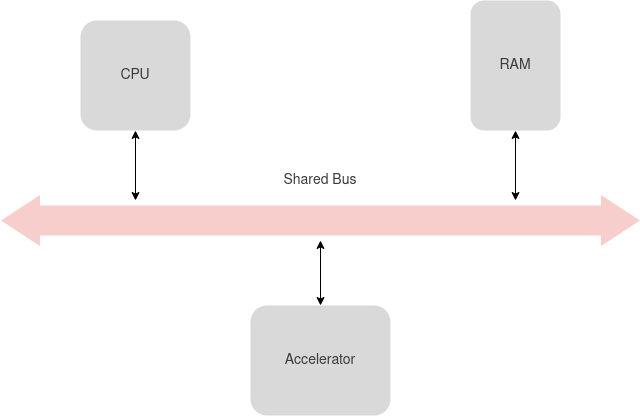
\includegraphics[width=8cm]{Images/Overview-Overview.png}
\caption{\content Overview of the system.}
\end{figure}
\nointend The principal objective of our project is to design vector accelerators for elementwise negation and statistics minima. These accelerators are connected to a common bus and have directory access to the memory, further lessening the CPU workload. The CPU issues instructions to the accelerators, which comprises pointers to data in the memory. There is no direct data transfer between the CPU and the accelerators. The result of the vector computation is written back to the memory. The Control Status Registers in these accelerators let the CPU control and read status from them. Vector instructions on float32, int8, int16 & int32 data types are implemented. 
\section*{Parameterized and Modular Design\sdot}
Our design is completely modular. All the modules, i.e., the CPU, Memory, and Accelerators, are parameterized. All the modules can be instantiated with many different combinations of parameters, including wordlength, data length, and bus data \& address width subjected to logical constraints.

\section*{Testbench, Simulation and Custom Assembler\sdot}

To ease the development process with better testing capabilities, we wrote a minimal assembler in Python that converts the sequences of instructions supported by our CPU into machine code, which can be utilized to initialize the instruction memory in Bluespec.\\
\begin{figure}[H]
\centering
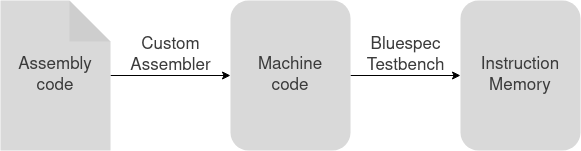
\includegraphics[width=8cm]{Images/Overview-Simulation.png}
\caption{\content Simulation of the system.}
\end{figure}
\noindent For more details about the instruction set, see section CPU.
\end{paper}
\contribution{Central Processing Unit}
\shortcontributor{CS6230 : CAD for VLSI Project Report}
\shortcontribution{Overview}
\headnum{2}
\begin{paper}
\renewcommand*{\pagemark}{}

\section*{}


\begin{figure}[H]
\centering
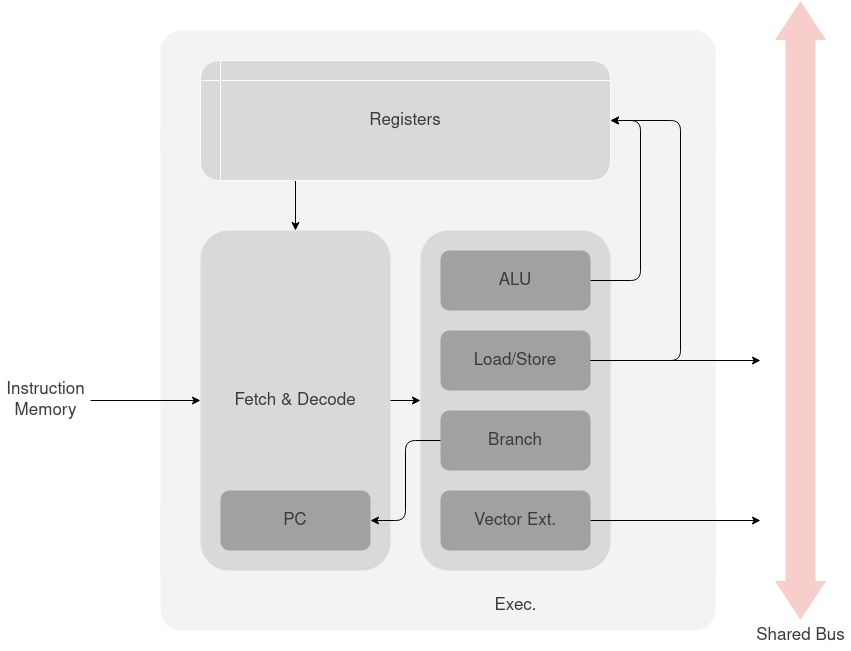
\includegraphics[width=10cm]{Images/Overview-CPU(1).png}
\caption{\content Architecture of the CPU.}
\end{figure}

\nointend We designed a minimal 2 stage pipelined CPU capable of doing basic arithmetic, logic, memory load/store, and custom vector operations. The instruction memory is separated from the data memory. Instructions will be issued in order. For branches, the fetch stage will be flushed, and the program counter will be updated. In the case of vector instructions, the appropriate CSRs of the corresponding accelerators will be updated accordingly. The general architecture of the CPU is as given in the figure.
\section*{The Registers\sdot}
Our CPU consists of 8 general-purpose registers R0, R1, R2, ... R7. The capacity of the registers is parameterized. However, our current instruction set supports only 8, 16, and 32-bit values and operations on them. According to the instruction, an individual physical register can be perceived as an 8-bit, a 16-bit, or a 32-bit register. For instance, \texttt{ASG\_8 R1 4} will consider only the lower 8 bits of R1, whereas \texttt{ASG\_15 R1 4} will consider the lower 16 bits.
\begin{figure}[H]
\centering
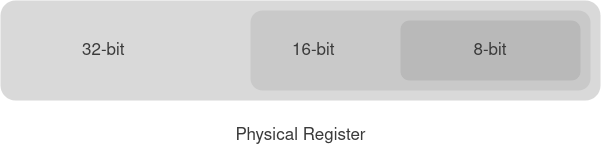
\includegraphics[width=8cm]{Images/Overview-Registers.png}
\caption{\content The same register RX can be perceived as 8, 16 or 32-bit register.}
\end{figure}

\section*{The Instruction Set\sdot}
\begin{figure}[H]
\centering
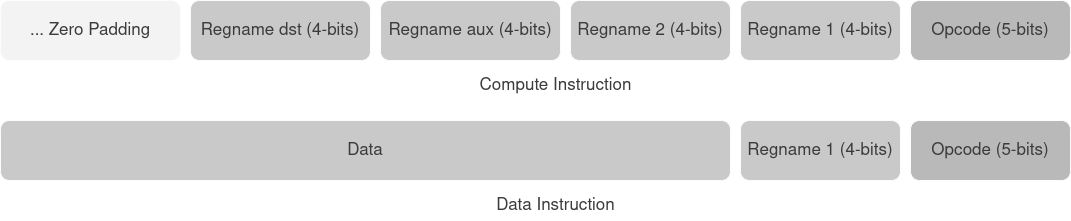
\includegraphics[width=11cm]{Images/Overview-InstructionSet.png}
\caption{\content Structure of the instructions.}
\end{figure}
We devised a minimal custom ISA capable of basic arithmetic, logic, branch, load/store, and custom vector operations. The CPU's must have a minimum word length of 32 bits. The same instructions, padded with zeros, are used for CPUs of higher word lengths. All instructions except the 32-bit Assign instruction in 32-bit CPUs are of the same length equal to the word length. In this case, the instruction (\texttt{ASG\_32} in 32-bit CPU) is 64-bits long to accommodate the 32-bit value for Assign operation. Our custom ISA is as given below. A small assembler was written in Python to generate machine code in a format supported by Bluespec testbench.\\\\
\nointend To run the assembler,
\begin{minted}[
bgcolor=Gray !20
]{bash}
cd src/asm/
./asm input_file.asm -o output -w 64
\end{minted}
\nointend Where the \texttt{-w} argument is the wordlength of the CPU. The argument is optional and the default is as for a 32-bit CPU.


\begin{center}
\begin{longtable}{l l l l}
 \heavy Instruction & \heavy Opcode& \heavy Example & \heavy Description\\ 
NOP & 0x00 & NOP & No op \\  
ASG\_8 & 0x01 & AGS\_8 R1 11 & Assigns int8 11 to Register R1 \\
ASG\_16 & 0x02 & ASG\_16 R1 11 & Assigns int16 int 11 to Register R1 \\
ASG\_32 & 0x03 & ASG\_32 R1 11 & Assigns int32 int 11 to Register R1 \\
&&ASG\_32 R1 11.0 & Assigns float32 11.0 to Register R1 \\
MOV & 0x04 & MOV R1 R2 & Moves content of R1 to R2\\
ADD\_I8 & 0x05 & ADD\_I8  R1 R2 R3 & int8 addition R3 <- R1 + R2\\
ADD\_I16 & 0x06 & ADD\_I16  R1 R2 R3 & int16 addition R3 <- R1 + R2\\
ADD\_I32 & 0x07 & ADD\_I32  R1 R2 R3 & int32 addition R3 <- R1 + R2\\
ADD\_F32 & 0x08 & ADD\_F32  R1 R2 R3 & float32 addition R3 <- R1 + R2\\
SUB\_I8 & 0x09 & SUB\_I8  R1 R2 R3 & int8 addition R3 <- R1 + R2\\
SUB\_I16 & 0x0a & SUB\_I16  R1 R2 R3 & int16 addition R3 <- R1 - R2\\
SUB\_I32 & 0x0b & SUB\_I32  R1 R2 R3 & int32 addition R3 <- R1 - R2\\
SUB\_F32 & 0x0c & SUB\_F32  R1 R2 R3 & float32 addition R3 <- R1 - R2\\
IS\_EQ & 0x0d & IS\_EQ  R1 R2 R3 & R3 <- (R1 == R2)\\
JMP & 0x0e & JMP R1 & Jump PC to address pointed by R1\\
JMPIF & 0x0f & JMPIF R1 R2 & Jump to address R1 if R2 is true\\
LOAD\_8 & 0x10 & LOAD\_8 R1 R2 & Load 8-bits from address pointed\\
&&& by R1 to R2\\
LOAD\_16 & 0x11 & LOAD\_16 R1 R2 & Load 16-bits from address pointed\\
&&& by R1 to R2\\
LOAD\_32 & 0x12 & LOAD\_32 R1 R2 & Load 32-bits from address pointed\\
&&& by R1 to R2\\
STORE\_8 & 0x13 & STORE\_8 R1 R2 & Store 8-bits R1 to address pointed\\
&&& by R2\\
STORE\_16 & 0x14 & STORE\_16 R1 R2 & Store 16-bits R1 to address pointed\\
&&& by R2\\
STORE\_32 & 0x15 & STORE\_32 R1 R2 & Store 32-bits R1 to address pointed\\
&&& by R2\\
VEC\_NEG\_I8 & 0x16 & VEC\_NEG\_I8 R1 R2 R3 & Bit wise negation of int8 vector\\
&&& starting pointed by R1, length R2,\\
&&& and store back to address in R3\\
VEC\_NEG\_I16 & 0x17 & VEC\_NEG\_I16 R1 R2 R3 & Bit wise negation of int16 vector\\
&&& starting pointed by R1, length R2,\\
&&& and store back to address in R3\\
VEC\_NEG\_I32 & 0x18 & VEC\_NEG\_I31 R1 R2 R3 & Bit wise negation of int32 vector\\
&&& starting pointed by R1, length R2,\\
&&& and store back to address in R3\\
VEC\_NEG\_F32 & 0x19 & VEC\_NEG\_F32 R1 R2 R3 & Bit wise negation of float32 vector\\
&&& starting pointed by R1, length R2,\\
&&& and store back to address in R3\\
VEC\_MIN\_I8 & 0x1a & VEC\_MIN\_I8 R1 R2 R3 & Statistics minimum of int8 vector\\
&&& starting pointed by R1, length R2,\\
&&& and store back to address in R3\\
VEC\_MIN\_I16 & 0x1b & VEC\_MIN\_I16 R1 R2 R3 & Statistics minimum of int16 vector\\
&&& starting pointed by R1, length R2,\\
&&& and store back to address in R3\\
VEC\_MIN\_I32 & 0x1c & VEC\_MIN\_I31 R1 R2 R3 & Statistics minimum of int32 vector\\
&&& starting pointed by R1, length R2,\\
&&& and store back to address in R3\\
VEC\_MIN\_F32 & 0x1d & VEC\_MIN\_F32 R1 R2 R3 & Statistics minimum of float32 vector\\
&&& starting pointed by R1, length R2,\\
&&& and store back to address in R3\\
\end{longtable}
\end{center}


\section*{The Fetch and Decode Stage\sdot}
The fetch stage fetches the instructions from the instruction memory, checks for any data dependencies, and looks up the data required for computation from the registers, and enqueues to decoded instruction to the execute stage. In the case of any data dependencies, a \texttt{NOP} is sent into the execute stage. \\\\
\nointend All the data instructions (the assignment instructions) are processed in the fetch stage. This architecture creates a conflict if the execute stage tries to store a value to the same register. The data instruction from the fetch stage is given priority for resolving the conflict. In other words, during a consecutive write after write (WAW) dependency, the first write is disregarded.\\\\
\nointend The fetch stage is also responsible for decomposing complex vector instructions to a sequence of load/store instructions. For example, the \texttt{VEC\_NEG\_I8} instruction is broken down into a stream of store instructions that stores the pointers to the data to the memory-mapped accelerator and triggers the accelerator. This process creates overhead on the CPU. A potential alternative is for the compiler to decompose the vector functions and keep the individual instructions short. However, this method results in more large programs. 

\section*{The Execute Stage\sdot}
Since being an inorder processor, the execute stage is relatively straight forward. The opcode is used to send the instructions to the right unit. In the case of a branch, the pipeline is flushed. There is no value forwarding to the fetch stage, and the instructions with data dependencies are kept awaiting. There is also no value forwarding between store and load operations. \\\\
\nointend For vector instructions, the fetch stage already decomposes the instructions into the corresponding load/store transactions. Therefore the execute stage executes these instructions, idles and pings the accelerator to check for the completion of the instruction. The length of the vector determines the frequency of pings. The pings must not be excessively frequent as it consumes the expensive bus ownership time that the accelerators require, and the pings must not be over sparse as this results in the CPU holding idle for long.
\end{paper}
\contribution{Random Access Memory}
\shortcontributor{CS6230 : CAD for VLSI Project Report}
\shortcontribution{Overview}
\headnum{3}
\begin{paper}
\renewcommand*{\pagemark}{}

\section*{}
Memory access is the bottleneck in almost all of the vector operations. A multi-ported RAM with parallel read/writes coupled with a wide data bus is essential to profit from the vector accelerators' parallel processing capabilities.
\section*{Implimentation\sdot}
Vectors of EHRs were used to implement the RAM. CReg supplied by Bluespec limited the number of ports to 5. Assuming the smallest addressable unit is 1 byte (this is parameterized in the implementation), this limitation caused the throughput to be capped at 5 bytes per cycle. Another implementation of EHRs from {\color{RubineRed} https://web.mit.edu/6.375/install/bsvclib-2007-02-20\_19-10/EHR.bsv} removed this limitation, and the memory throughput is now only limited by the bus width. The ports followed the priority rules of EHRs. A wrapper was written to coordinate the ports and interface with the bus. To illustrate, if the bus requested only 1 byte, only one port would be active. On the other case, if the bus can transmit 64 bytes per cycle (512 bits) and requests for 512 bits, all 64 ports would be active.
\begin{figure}[H]
\centering
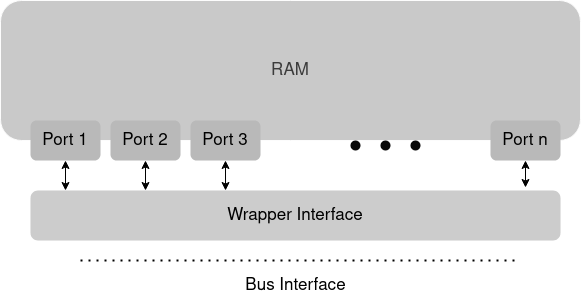
\includegraphics[width=7cm]{Images/Overview-Ram.png}
\caption{\content Ram wrapper interfaces bus to the ports.}
\end{figure}
\end{paper}
\contribution{The Bus}
\shortcontributor{CS6230 : CAD for VLSI Project Report}
\shortcontribution{Overview}
\headnum{4}
\begin{paper}
\renewcommand*{\pagemark}{}

\section*{}
Although Bluespec provides a Config bus (CBus) interface through the CBus and LBus package, top-level test benches have to be written to mediate communication between two or more module interfaces. Employing the CBus package hindered modularity as we insisted our modules to have plug and play interfaces. Bluespec also had implemented in their libraries many of the standard bus protocols like AHB and AXI with TLM interface. These provided full-fledged capabilities that were overkill for use in our system. So, we decided on a simple bus protocol to implement ourselves on Bluespec.
\section*{The Bus System\sdot}
\begin{figure}[H]
\centering
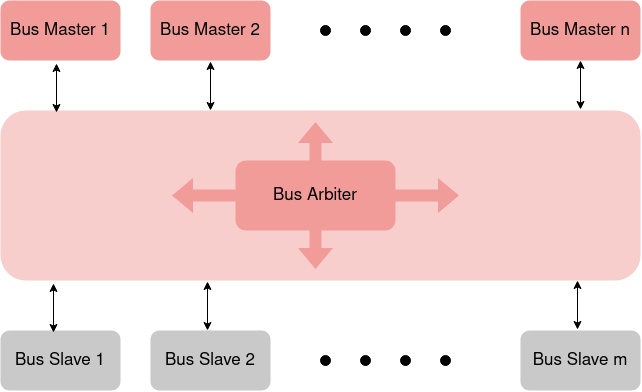
\includegraphics[width=8cm]{Images/Overview-Bus.png}
\caption{\content The bus system.}
\end{figure}\\
\nointend The system consists of a Bus Fabric to which different modules are connected. There are two types of modules, the Bus Masters and the Bus Slaves. Masters issue read or write requests to which slaves have to respond if the requested address is within its scope. The bus Arbiter determines which master owns the bus. Before sending a request, all masters must request the Arbiter. In the case of multiple requests, the Arbiter uses round-robin scheduling to select the owner of the bus. We used Bluespec's \texttt{Arbiter} package for implementing the Arbiter.
\section*{The Bus Protocol\sdot}
\begin{figure}[H]
\centering
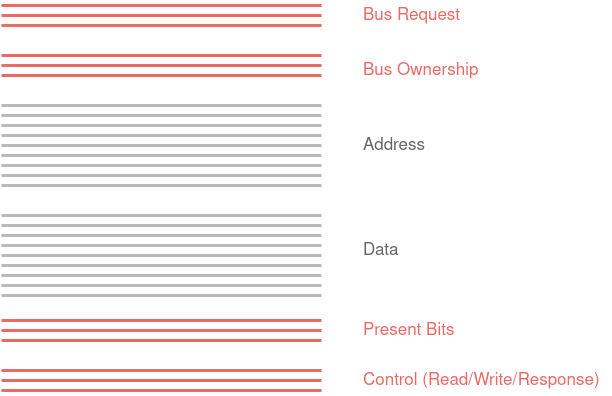
\includegraphics[width=8cm]{Images/Overview-BusWires.png}
\caption{\content The bus wires.}
\end{figure}\\
\nointend Every master gets assigned two exclusive lines, one for requesting the Arbiter and another to receive the Arbiter response. All the rest of the Bus lines are shared.\\\\
\nointend A read request consists of an Address, the present bits indicating the number of units of the smallest addressable blocks expected by the sender, and the control wires in 'Read' mode. For example, to request four consecutive bytes to a RAM whose smallest addressable unit is 1 byte, we have our present bits to have a value of 4. In this way, connected slaves can utilize the entire bus width to the maximum. Similarly, a write request consists of almost the same details except for the data and control in 'Write' mode. Slaves respond with the appropriate 'Response.'
\section*{Interfacing the Bus\sdot}
The BusMaster and BusSlave modules provide an effortless bridge between the Bus and the associated components. Read/write requests can be enqueued into the BusMaster, and responses can be read using simple GetPut interfaces. Corresponding interfaces also exist towards the BusSlaves.
\begin{figure}[H]
\centering
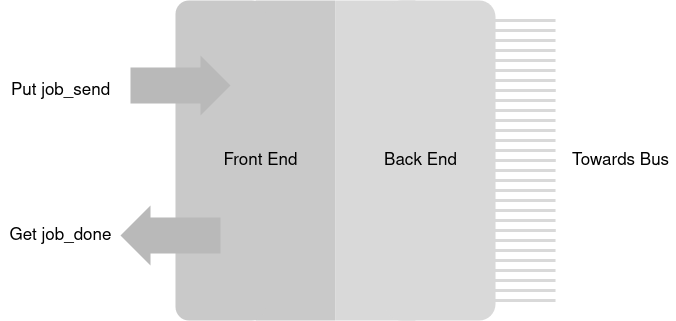
\includegraphics[width=8.8cm]{Images/Overview-BusMaster.png}
\caption{\content The BusMaster.}
\end{figure}
\begin{figure}[H]
\centering
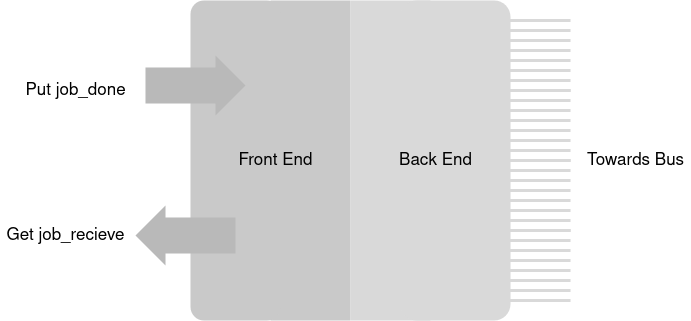
\includegraphics[width=9cm]{Images/Overview-BusSlave.png}
\caption{\content The BusSlave.}
\end{figure}\\
\nointend For details about using the Bus, see the documentation section.
\end{paper}

\part[Vector Extensions]{Vector Extensions\sdot}
\contribution{A Brief Introduction }
\shortcontributor{CS6230 : CAD for VLSI Project Report}
\shortcontribution{Vector Extensions}
\headnum{5}
\begin{paper}
\renewcommand*{\pagemark}{}
\section*{}
\begin{figure}[H]
\centering
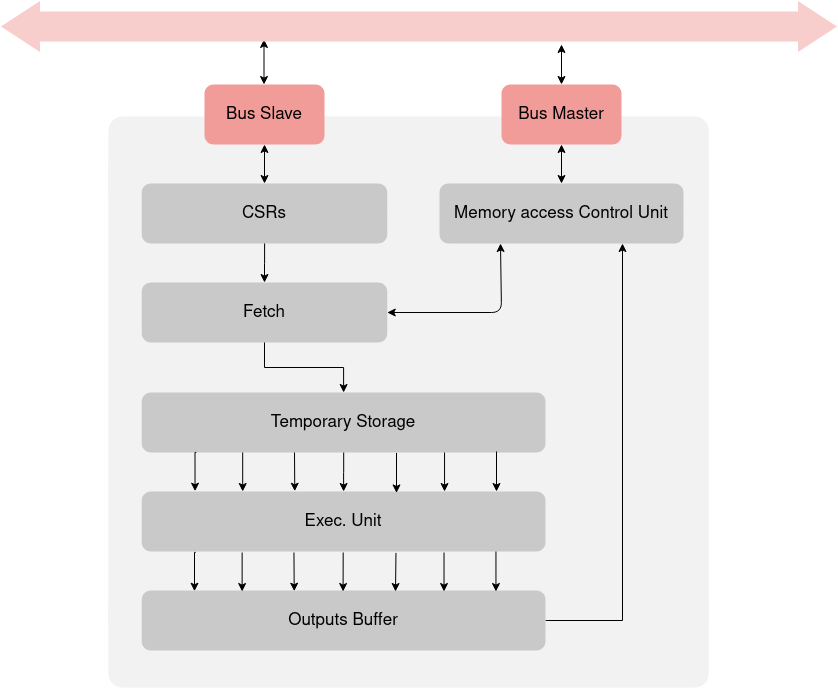
\includegraphics[width=11cm]{Images/VectorExtensions.png}
\caption{\content General architecture of our Vector Processing Unit.}
\end{figure}\\
\nointend The general architecture for a vector accelerator is as given in the figure. While such a formation is suitable for most vector operations, matrix operations may require a
different kind of design with systolic arrays. Since we intend to devise a design for accelerators concerning vector negation and statistics minimum, we restrict the general design for vector operations. It is to be remarked that slight alterations in dataflow may be required for binary vector operations.\\\\
\nointend The CPU writes the pointers for the source & destination vectors and the vector size into the accelerators' CSRs. Once the CPU instructs the accelerator to start computation by writing to the start flag of the CSRs, the fetch unit requests the memory access controller for the data. The memory access controller handles read/write requests and responses between the accelerator and the bus. The memory access controller uses round-robin scheduling for handling simultaneous read and write requests. Once the fetch unit gets the data corresponding to a portion of the vector, it gets enqueued onto the temporary storage unit.

\end{paper}
\contribution{The Control Status Registers}
\shortcontributor{CS6230 : CAD for VLSI Project Report}
\shortcontribution{Vector Extensions}
\headnum{6}
\begin{paper}
\renewcommand*{\pagemark}{}
\section*{}
The Control Status Registers (CSRs) is the only communication path between the processor and the accelerator. There are multiple CSRs, each for a specific purpose. Each CSR has an exclusive address, as indicated in the figure given below. When the CPU encounters a vector instruction, it writes the required operands, i.e., the address of the source, block size of the vector, the Opcode, and the address where the result is to be stored into the CSRs. After these operands are written, the CPU writes one into the Start flag. This action causes the accelerator to start its operation. The Aux CSR is used for any extra data required by any new functionality. This design helps in adding functionality without significantly altering the design. For instance, the pointer to the minima index in vector neg operation utilizes the Aux register.\\
\begin{figure}[H]
\centering
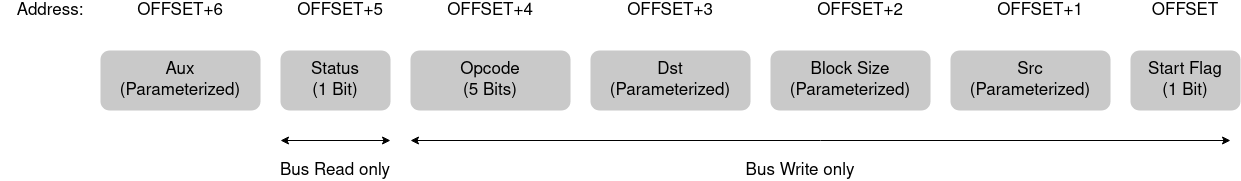
\includegraphics[width=\textwidth]{Images/VectorExtensions-CSRUniary(1).png}
\caption{\content Control status Registers for a Unary Vector Extension.}
\end{figure}

\noindent There is also a 1-Bit status register, which, when equals one, means that the accelerator has completed its operation and is idle.
\section*{Interface with the Bus\sdot}
The CSRs interface the Bus through a BusSlave. This means that CSRs cannot launch a request by themselves. The CSR's can only respond to read/write requests initiated by the processor or any other masters. So the CPU must periodically ping the accelerator to know the status of any operation previously initiated. The \textttt{Start Flag, Src, Block Size, Dst, and Opcode} are write-only. A null response is returned if the CPU attempts to read them. Similarly, the CPU can only read the \texttt{Status} register. Any attempts to write is ignored.

\end{paper}
\contribution{The Vector Fetch Unit}
\shortcontributor{CS6230 : CAD for VLSI Project Report}
\shortcontribution{Vector Extensions}
\headnum{7}
\begin{paper}
\renewcommand*{\pagemark}{}

\section*{}
The vector accelerator's degree of parallelism is upper bounded by the width of the data bus. The fetch unit breaks down a vector into parts of this size and get the data from memory sequentially. The data request is made through the Memory access Control Unit. For instance, suppose the data bus's width is 512 bits, and the vector units can support 512 bits; the degree of parallelism is 64 elements for 8-bit ints, 32 elements for 16-bit, and 16 elements for 32-bit floats \& ints. The fetched data is enqueued to a temporary storage unit from where the data goes to a pipelined execution unit.

\section*{Temporary Storage Units\sdot}
\begin{figure}[H]
\centering
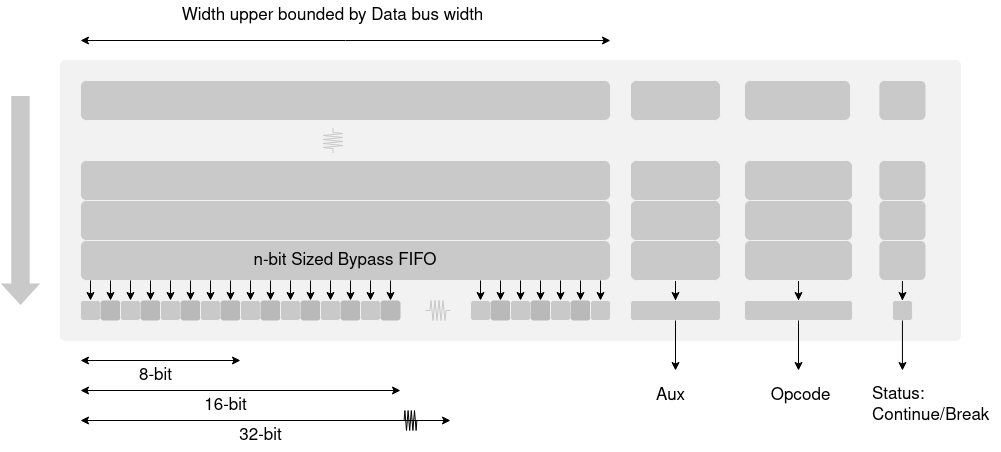
\includegraphics[width=\textwidth]{Images/VectorExtensions-temp_structure(2).png}
\caption{\content Structural view of the temporary storage units}
\end{figure}\\
\nointend The temporary storage unit is constructed out of Bypass FIFOs. Bluespec does not support the construction of sized Pipeline FIFOs, but similar functionality can be obtained by having a Pipeline FIFO in series with a sized Bypass FIFO. The outputs can be deciphered according to the Opcode and can be gathered by the appropriate execution unit. The width of the complete unit depends on the highest bandwidth supported through the bus. The functional representation of such a unit is manifested in the following figure.
\begin{figure}[H]
\centering
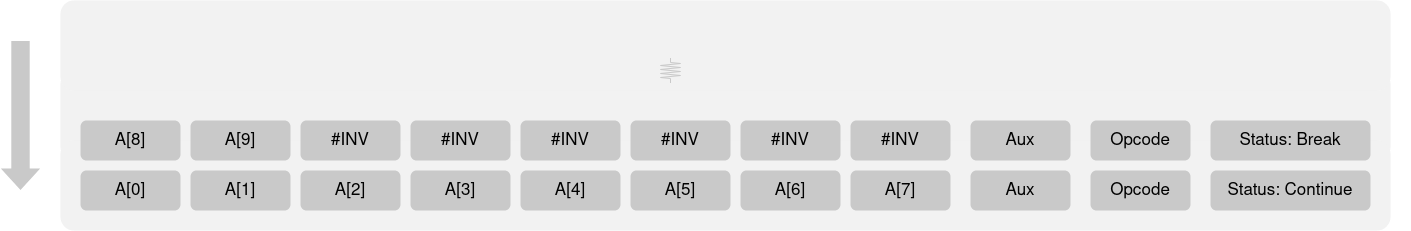
\includegraphics[width=\textwidth]{Images/VectorExtensions-temp-func(1).png}
\caption{\content Functional view of a 64-bit wide storage unit storing a vector of int8 A[10]}
\end{figure}


\end{paper}
\contribution{The Vector Execute Units}
\shortcontributor{CS6230 : CAD for VLSI Project Report}
\shortcontribution{Vector Extensions}
\headnum{8}
\begin{paper}
\renewcommand*{\pagemark}{}

\section*{}
The data from the temporary storage units arrive at the right execute units designated by the Opcode through a Pipeline FIFO. The architecture of the two main vector functions that we focus on in this project is given below.
\section*{Vector Negation\sdot}
Implementing elementwise vector negation was relatively straight forward as there is only one to one correspondence between the inputs and outputs. For integers in 2's complement representation, negation is achieved by inverting all numbers and adding one. However, the abstraction level provided by the implementation of integers in Bluespec libraries hides all details from the writer and can be written directly. \\\\
\nointend For floating-point values, merely flipping the sign bit of a value results in the number's negative. We employed Bluespec's \texttt{FloatingPoint} library, which provided direct arithmetic functionality.
\section*{Vector Statistics Minima\sdot}
The statistics minima operation is devised to run in logarithmic time complexity. Since every vector is of variable length, usually longer than the execution unit's width, we were required to maintain the system's state. The state contains the value of the minimum from the previous batch. The state is updated if the current batch's minimum is less than the minimum of the previous batch. A status signal of 'Break' resets the states. The indices of the minima are also calculated concurrently along with the minima.
\begin{figure}[H]
\centering
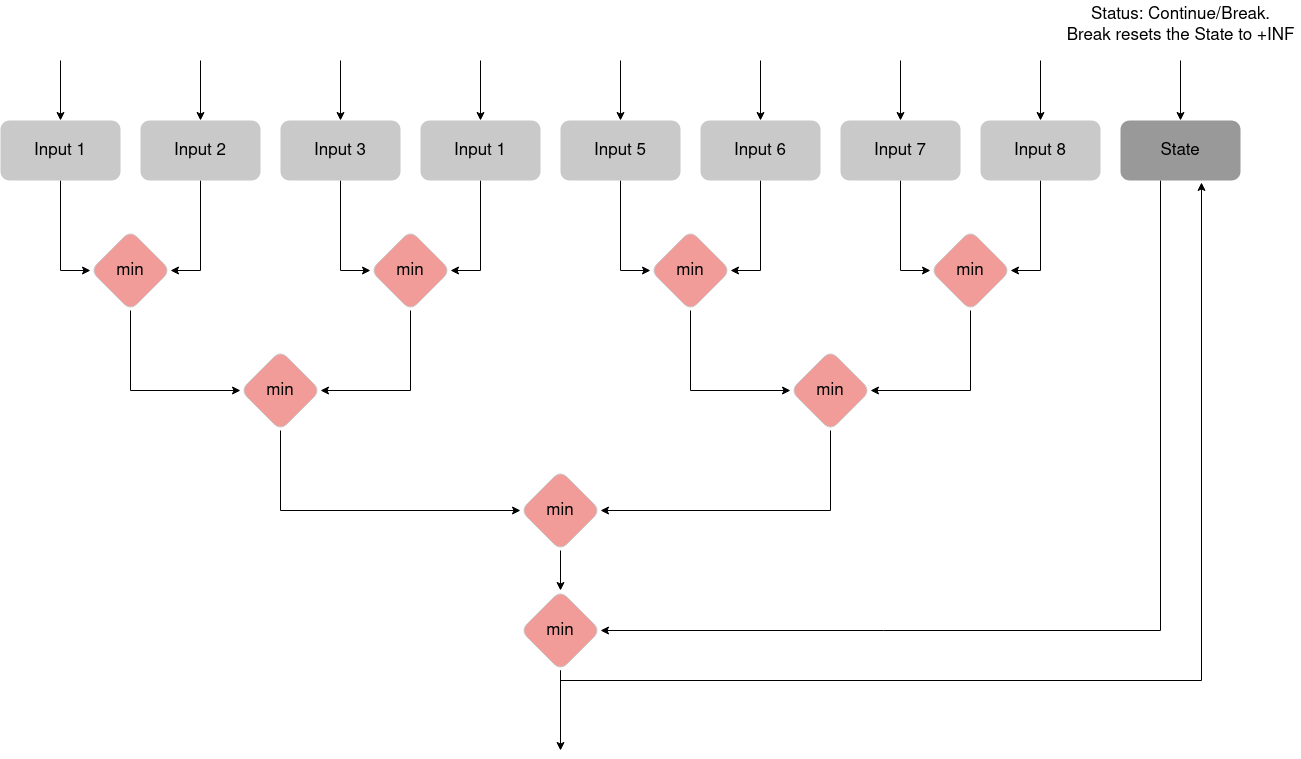
\includegraphics[width=\textwidth]{Images/VectorExtensions-minima.png}
\caption{\content Execute unit for computing statistics minima.}
\end{figure}


\end{paper}

\part[Demo]{Demo\sdot}
\contribution{CPU Demo, The Fibonacci Series}
\shortcontributor{CS6230 : CAD for VLSI Project Report}
\shortcontribution{Demo}
\headnum{9}
\begin{paper}
\renewcommand*{\pagemark}{}

\section*{}
To demonstrate the capabilities of the CPU and the accelerator, we have included a few demo test benches. These can be run from \texttt{src/Demo/Demo.bspec}. There are 2 bsv test benches, \texttt{Demo1.bsv and Demo2.bsv}. \texttt{Demo1.bsv} contains only the CPU whereas \texttt{Demo2.bsv} contains both CPU and the accelerator. 

\section*{The Assembly Code\sdot}
The assembly code for printing the first ten elements of the CPU is located in \texttt{src/asm/fibonacci\_asm.asm}. The code snippet is as given below.
\begin{minted}[
bgcolor=Gray !5,
escapeinside=||
]{nasm}
NOP                     ; A test code to print that prints the Fibonacci series
ASG_32 R7 128           ; Assign the address of the console
ASG_32 R1 1             ; Initialize first two elements
ASG_32 R2 1             ;
ASG_32 R6 8             ; Loop count. Print 10 (first 2 + 8)  
ASG_32 R5 0             ; Loop initialise
ASG_32 R4 1             ; Loop increment
STORE_32 R1 R7          ; Print first 2 values through memory mapped console
STORE_32 R2 R7          ;
loop: ADD_I32 R1 R2 R3       ; Calculate the next element
    ASG_32 R7 128            ; Assign the console address again
    STORE_32 R3 R7           ; Print the new term
    MOV R2 R1                ; Forget the past and move ahead
    MOV R3 R2                ; 
    ADD_I32 R5 R4 R5         ; Loop increment          
    IS_EQ R5 R6 R3           ; 
    ADD_I32 R3 R4 R3         ; IS_EQ outputs 1 if true. But we need 1 to jump.  
    ASG_32 R7 |\$|loop          ; Jump branch destination      
    JMPIF R7 R3              ; Conditional Jump
\end{minted}\\\\
\nointend To generate machine code run,
\begin{minted}[
bgcolor=Gray !5
]{bash}
cd src/asm
./asm fibonacci_asm.asm -o fibonacci -w 64
\end{minted}\\\\
\nointend Here \texttt{-o fibonacci} is the output file name and \texttt{-w 64} tells the assembler than we are generating code for a 64-bit machine.\\\\
\nointend To run the simulation, execute,
\begin{minted}[
bgcolor=Gray !5
]{bash}
cd src/Demo
./compile_and_sim.sh Demo1.bsv
\end{minted}\\\\
\nointend If you have already compiled once, just run,
\begin{minted}[
bgcolor=Gray !5
]{bash}
cd src/Demo
./out
\end{minted}\\\\
\nointend If no errors occur, you will get the final outputs as,
\begin{minted}[
bgcolor=Gray !5,
breaklines
]{bash}
...
Running ./out
Warning: file '../asm/fibonacci' for memory 'my_core_imem_c_memory' has a gap at addresses 19 to 18446744073709551615.
CONSOLE 00000001 |           1
CONSOLE 00000001 |           1
CONSOLE 00000002 |           2
CONSOLE 00000003 |           3
CONSOLE 00000005 |           5
CONSOLE 00000008 |           8
CONSOLE 0000000d |          13
CONSOLE 00000015 |          21
CONSOLE 00000022 |          34
CONSOLE 00000037 |          55

\end{minted}\\\\
\section*{Looking at Demo1.bsv\sdot}
Here is a snippet from \texttt{Demo1.bsv} that specifies the machine parameters.
\begin{minted}[
bgcolor=Gray !5
]{haskell}
`define WORD_LENGTH 64  // We are making a 64 bit machine
`define DATA_LENGTH 32  // The data size of our machine
`define BUS_DATA_LEN 32 // Data bus width
`define ADDR_LENGTH 20  // Addr bus width

`define GRANULARITY 8   // Smallest addressible unit (1 Byte at every address)
`define RAM_BYTES 64    // Ram size (number of addressible units)
`define RAM_PORTS 4     // 4 ports, 4 x 8 for 32 bit bus

`define RAM_ADDRESS_OFFSET 1000 // Address of the RAM
`define CONSOLE_ADDRESS 128     // Address of the Console
\end{minted}\\\\
\nointend The console is just a slave connected to the bus that prints everything written to its address. It is made only for debugging purposes. Notice that we are writing to address 128 in the above assembly code to print the value.
\begin{minted}[
bgcolor=Gray !5
]{haskell}
CPU #(`WORD_LENGTH,
      `DATA_LENGTH, 
      `BUS_DATA_LEN, 
      `ADDR_LENGTH, 
      `GRANULARITY) 
      my_core <- mkCPU(1, "../asm/fibonacci"); // CPU_ID 1, Initialize IMEM
\end{minted}\\\\
\nointend We transfer the generated machine code to the CPU to initialize the instruction memory while instantiating.
\begin{minted}[
bgcolor=Gray !5
]{haskell}
DRAMSlave #(`GRANULARITY, 
            `RAM_BYTES, 
            `RAM_ADDRESS_OFFSET, 
            `BUS_DATA_LEN, 
            `ADDR_LENGTH,
            `RAM_PORTS) my_dram    <- mkDRAMSlave(0);

Console #(`BUS_DATA_LEN,
          `ADDR_LENGTH,
          `GRANULARITY)      my_console <- mkConsole(1, `CONSOLE_ADDRESS);

Vector #(1, BusMaster #(`BUS_DATA_LEN, 
                        `ADDR_LENGTH, 
                        `GRANULARITY)) master_vec;

Vector #(2, BusSlave  #(`BUS_DATA_LEN, 
                        `ADDR_LENGTH, 
                        `GRANULARITY)) slave_vec;


master_vec[0] = my_core.bus_master;
slave_vec[0]  = my_dram.dram_slave;
slave_vec[1]  = my_console.bus_slave;

Bus #(1, 2,             // 1 master, 2 slaves
      `BUS_DATA_LEN, 
      `ADDR_LENGTH, 
      `GRANULARITY) bus <- mkBus(master_vec, slave_vec);

mkConnection (master_vec, bus);
mkConnection (slave_vec, bus);
\end{minted}\\\\
\nointend Here you can see how all BusMaster and BusSlave interfaces are connected to the main Bus. The vectors of all BusMasters and Slaves are passed to the \texttt{mkBus(..)}. Also \texttt{mkConnection (..)} is used to connect the interfaces. \\\\
\end{paper}
\contribution{Demo, Vector Negate}
\shortcontributor{CS6230 : CAD for VLSI Project Report}
\shortcontribution{Demo}
\headnum{10}
\begin{paper}
\renewcommand*{\pagemark}{}

\section*{}
In this demo, we will be generating a 32-bit CPU and attach it with a vector accelerator. \texttt{src\Demo\Demo2.bsv} contains the required setup concerning this. 
\section*{Looking at Demo2.bsv\sdot}
\texttt{Demo2.bsv} is different from \texttt{Demo1.bsv}. It contains our vector accelerator attached to the Bus.
\begin{minted}[
bgcolor=Gray !5,
breaklines
]{haskell}
`include <VX_Address.bsv> // Location where Accelerator is memory mapped

`define WORD_LENGTH 32   // Here we are generating a 32 bit CPU
`define DATA_LENGTH 32
`define BUS_DATA_LEN 128 // When changing bus width, remember to increase memory ports 
`define ADDR_LENGTH 20
`define VECTOR_DATA_SIZE `BUS_DATA_LEN
`define VX_STORAGE_SIZE 2

`define GRANULARITY 8    // Smallest addressible unit (1 byte)
`define RAM_BYTES 64     // Ram size (number of addressible units)
`define RAM_PORTS 16     // 16 ports, 1 byte per port for 128 bit bus
`define RAM_ADDRESS_OFFSET 1024

`define CONSOLE_ADDRESS 128
\end{minted}\\\\
\nointed The vector accelerator is defined as attached as follows,
\begin{minted}[
bgcolor=Gray !5,
breaklines
]{haskell}
VectorUnary #(`DATA_LENGTH,
               `VECTOR_DATA_SIZE,
               `BUS_DATA_LEN,
               `ADDR_LENGTH,
               `GRANULARITY) vec_Unary <- mkVectorUnary (`VX_ADDRESS, `VX_STORAGE_SIZE, 7);
                                        // VX_ADDRESS <- Memory mapped address of Accelerator
                                        // VX_STORAGE_SIZE <- Depth of temporary storage FIFOs
Vector #(2, BusMaster #(`BUS_DATA_LEN, 
                        `ADDR_LENGTH, 
                        `GRANULARITY)) master_vec;

Vector #(3, BusSlave  #(`BUS_DATA_LEN, 
                        `ADDR_LENGTH, 
                        `GRANULARITY)) slave_vec;

...
...
...

slave_vec[2]  = vec_Unary.bus_slave;

Bus #(2, 3, `BUS_DATA_LEN, 
            `ADDR_LENGTH, 
            `GRANULARITY) bus <- mkBus(master_vec, slave_vec);

mkConnection (master_vec, bus);
mkConnection (slave_vec, bus);

\end{minted}\\\\
\section*{Running Demo Files\sdot}
Four separate assembly files are provided for demonstrating vector negation on four different datatypes, \texttt{int8, int16, int32 & float32}. These files are located at,
\begin{minted}[
bgcolor=Gray !5,
breaklines
]{text}
src/asm/vec_neg_f32_demo.asm
src/asm/vec_neg_i8_demo.asm
src/asm/vec_neg_i16_demo.asm
src/asm/vec_neg_i32_demo.asm
\end{minted}\\\\
\nointend Here is a snippet of \texttt{src/Demo/vec\_neg\_i32\_demo.asm}. It initializes a vector of \texttt{int\_32}, of length 10 with numbers from 0 to 9. Vector negation is done and the output is printed. 

\begin{minted}[
bgcolor=Gray !5,
breaklines,
escapeinside=||
]{asm}
ASG_32 R1 0         ; Initialisation
ASG_32 R2 10        ; Num loops
ASG_32 R3 1024      ; Address
ASG_32 R4 1         ; Value increment delta
ASG_32 R5 4         ; Address increment delta
ASG_32 R0 128       ; Address of console
loop_init: STORE_32 R1 R3      ;
    STORE_32 R1 R0      ; Print console
    ADD_I32 R1 R4 R1    ; Increment value
    ADD_I32 R3 R5 R3    ; Increment address
    ASG_32 R7 1
    IS_EQ R1 R2 R6      ; Compare
    ADD_I32 R6 R7 R6
    ASG_32 R7 |\$|loop_init
    JMPIF R7 R6         ; Jump if not Eq
ASG_32 R3 1024
VEC_NEG_I32 R3 R2 R3    ; Vector negation
ASG_32 R1 0
loop_print: LOAD_32 R3 R4   ; Load from memory
    STORE_32 R4 R0          ; Print
    ADD_I32 R3 R5 R3        ; Incement address
    ASG_32 R4 1
    ADD_I32 R1 R4 R1        ; Increment Loop
    ASG_32 R7 1
    IS_EQ R1 R2 R6          ; Compare
    ADD_I32 R6 R7 R6
    ASG_32 R7 |\$|loop_print
    JMPIF R7 R6             ; Jump if not Eq
\end{minted}\\\\

\section*{Running the Simulation\sdot}
Generate machine code by running, 
\begin{minted}[
bgcolor=Gray !5,
breaklines
]{bash}
cd /src/asm
./asm vec_neg_i32_demo.asm -o vector
\end{minted}\\\\
\nointend Since, we are generating for a 32-bit CPU in this example, we do not have to specify the \texttt{-w N} option. 32-bit is the default value. Also note that the output file name is consistent with the input taken from \texttt{Demo2.bsv}\\\\
\nointend If compiling \texttt{Demo2.bsv} for the first time, run,
\begin{minted}[
bgcolor=Gray !5,
breaklines
]{bash}
cd src/Demo/
./compile_and_sim.sh Demo2.bsv 
\end{minted}\\\\
\nointend Else, if you have already compiled once, then run,
\begin{minted}[
bgcolor=Gray !5,
breaklines
]{bash}
cd src/Demo/
./out
\end{minted}\\\\
\nointend If no errors occur, you will get output similar to as shown below. Note that if you are running the demo on \texttt{float32}, the outputs are in IEEE 754 format hex and appear to not convey any legible information in \texttt{int}.
\begin{minted}[
bgcolor=Gray !5,
breaklines
]{bash}
CONSOLE 00000000 |           0
CONSOLE 00000001 |           1
CONSOLE 00000002 |           2
CONSOLE 00000003 |           3
CONSOLE 00000004 |           4
CONSOLE 00000005 |           5
CONSOLE 00000006 |           6
CONSOLE 00000007 |           7
CONSOLE 00000008 |           8
CONSOLE 00000009 |           9
CONSOLE 00000000 |           0
CONSOLE ffffffff |          -1
CONSOLE fffffffe |          -2
CONSOLE fffffffd |          -3
CONSOLE fffffffc |          -4
CONSOLE fffffffb |          -5
CONSOLE fffffffa |          -6
CONSOLE fffffff9 |          -7
CONSOLE fffffff8 |          -8
CONSOLE fffffff7 |          -9

\end{minted}\\

\end{paper}


\contribution{Demo, Statistics Minima}
\shortcontributor{CS6230 : CAD for VLSI Project Report}
\shortcontribution{Demo}
\headnum{11}
\begin{paper}
\renewcommand*{\pagemark}{}

\section*{}
In this demo, we will initialize a vector with some values, and we will print its minima and minimum index. The assembly files required for this demo are located at,
\begin{minted}[
bgcolor=Gray !5,
breaklines
]{text}
src/asm/vec_min_f32_demo.asm
src/asm/vec_min_i8_demo.asm
src/asm/vec_min_i16_demo.asm
src/asm/vec_min_i32_demo.asm
\end{minted}\\\\
\nointend Here is a snippet from \texttt{vec\_min\_i8\_demo.asm}
\begin{minted}[
bgcolor=Gray !5,
breaklines,
escapeinside=||
]{asm}
NOP                 ; Store Array [13, 12, 11, -13, 15]
ASG_32 R3 128       ; Console address
ASG_8 R1 13         ; Value
ASG_32 R2 1024      ; Address
STORE_8 R1 R2       ; Store to RAM
STORE_8 R1 R3       ; Print
ASG_8 R1 12         ; Value
ASG_32 R2 1025      ; Address
STORE_8 R1 R2       ; Store to RAM
STORE_8 R1 R3       ; Print
ASG_8 R1 11         ; Value
ASG_32 R2 1026      ; Address
STORE_8 R1 R2       ; Store to RAM
STORE_8 R1 R3       ; Print
ASG_8 R1 -13        ; Value
ASG_32 R2 1027      ; Address
STORE_8 R1 R2       ; Store to RAM
STORE_8 R1 R3       ; Print
ASG_8 R1 15         ; Value
ASG_32 R2 1028      ; Address
STORE_8 R1 R2       ; Store to RAM
STORE_8 R1 R3       ; Print
NOP
ASG_32 R1 1024      ; Vector starting location
ASG_32 R2 5         ; Vector size
ASG_32 R4 1024      ; Minimum dst
ASG_32 R5 1025      ; Argmin dst
VEC_MIN_I8 R1 R2 R4 R5  ; Vec op
LOAD_8 R4 R6        ; Load minima
STORE_8 R6 R3       ; Print minima
LOAD_8 R5 R7        ; Load argmin
STORE_8 R7 R3       ; Print argmin
\end{minted}\\\\

\section*{Running the Simulation\sdot}
Generate machine code by running, 
\begin{minted}[
bgcolor=Gray !5,
breaklines
]{bash}
cd /src/asm
./asm vec_min_i8_demo.asm -o vector
\end{minted}\\\\
\nointend Since, we are generating for a 32-bit CPU in this example, we do not have to specify the \texttt{-w N} option. 32-bit is the default value. Also note that the output file name is consistent with the input taken from \texttt{Demo2.bsv}\\\\
\nointend If compiling \texttt{Demo2.bsv} for the first time, run,
\begin{minted}[
bgcolor=Gray !5,
breaklines
]{bash}
cd src/Demo/
./compile_and_sim.sh Demo2.bsv 
\end{minted}\\\\
\nointend Else, if you have already compiled once, then run,
\begin{minted}[
bgcolor=Gray !5,
breaklines
]{bash}
cd src/Demo/
./out
\end{minted}\\\\
\nointend If no errors occur, you will get output similar to as shown below. Note that if you are running the demo on \texttt{float32}, the outputs are in IEEE 754 format hex and appear to not convey any legible information in \texttt{int}. The last 2 lines represent the minimum value and the index of the minimum value (starting from 0) respectively. If multiple minima exists, the index with the lower value is outputted.
\begin{minted}[
bgcolor=Gray !5,
breaklines
]{bash}
CONSOLE 0d |   13
CONSOLE 0c |   12
CONSOLE 0b |   11
CONSOLE f3 |  -13
CONSOLE 0f |   15
CONSOLE f3 |  -13
CONSOLE 03 |    3
\end{minted}\\
\end{paper}

\part[Documentation]{Documentation\sdot}
\contribution{Project Structure}
\shortcontributor{CS6230 : CAD for VLSI Project Report}
\shortcontribution{Documentation}
\headnum{12}
\begin{paper}
\renewcommand*{\pagemark}{}

\section*{Directory Structure\sdot}
\begin{wrapfigure}{R}{0.3\textwidth}
\centering
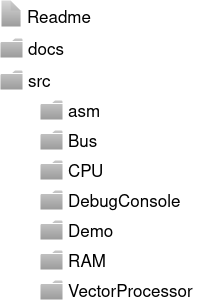
\includegraphics[width=0.3\textwidth]{Images/Overview-Dir.png}
\caption{\content The directory structure.}

\end{wrapfigure}

The directory structure of the project is as shown here. The directory \texttt{docs} contains all the documentation and its sources. The assembler and the sample assembly codes are present in the \texttt{asm} directory inside the \texttt{src}. The packages \texttt{Bus, CPU, DebugConsole, RAM and VectorProcessor} are located in their corresponding directories. The folder \texttt{Demo} contains the demo files demonstrating the usage and capablities.

\section*{Assembler\sdot} 
The assembler is located at the following path: \texttt{src/asm/asm}.

\section*{Demo Testbenches\sdot}
The demo testbenches are located at the following paths: \texttt{src/Demo/Demo1.bsv \& src/Demo/Demo2.bsv}

\section*{Git Repository\sdot}
The git repository of the project is located at the following url:\\ {\color{RubineRed}\url{https://github.com/Sooryakiran/Domain-Specific-Hardware-Accelerator-VLSI-CAD-Project/}}
\end{paper}



\contribution{Bus}
\shortcontributor{CS6230 : CAD for VLSI Project Report}
\shortcontribution{Documentation}
\headnum{13}
\begin{paper}
\renewcommand*{\pagemark}{}

\section*{Packages\sdot}
\texttt{import Bus :: * ;}
\section*{Description\sdot}
The Bus library includes interface, transactor, and function definition to fulfill a minimal Bus with Bluespec System Verilog. The implementation of BusMasters and Slaves can be attached to other devices employing naive Get and Put connections.

\begin{figure}[H]
\centering
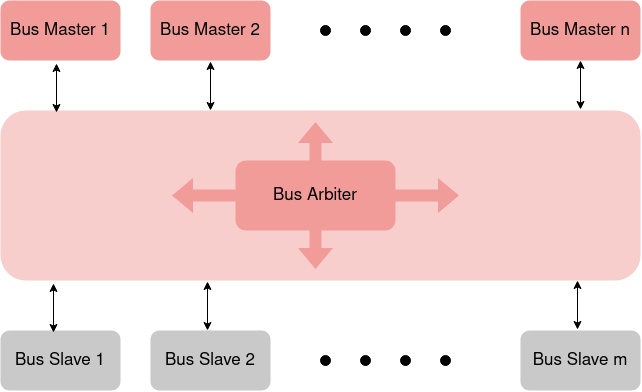
\includegraphics[width=8cm]{Images/Overview-Bus.png}
\caption{\content The bus system.}
\end{figure}\\


\section*{Data Structures\sdot}
Within the Bus, the data is composed of the following data structures: the \texttt{ControlSignal} contains information about the type of the signal, i.e, \texttt{Read, Write \& Response}. The \texttt{Chunk} datatype contains the entire signal.

\subsection*{Chunk\sdot}
The Chunk is a structure containing all the information to be transacted.

\begin{center}
\begin{longtable}{lll}
\multicolumn{3}{c}{\heavy Chunk\sdot}                                                      \\
\heavy Member  & \heavy Datatype                         & \heavy Valid Values        \\
control & ControlSignal                                  & Read/Write/Response \\
data    & Bit \#(datasize)                               & ..                  \\
addr    & Bit \#(addrsize)                               & ..                  \\
present & Bit \#(PresentSize \# (datasize, granularity)) & ..                 
\end{longtable}
\end{center}

\begin{minted}[
bgcolor=Gray !5
]{Haskell}
typedef enum {Response, Read, Write} ControlSignal deriving (Bits, Eq, FShow);

typedef TLog #(TAdd #(TDiv #(datasize, granularity), 1)) 
PresentSize #(numeric type datasize,
              numeric type granularity);

typedef struct {ControlSignal control;
                Bit #(datasize) data;
                Bit #(addrsize) addr;
                Bit #(PresentSize #(datasize, granularity)) present;}

                Chunk #(numeric type datasize,
                        numeric type addrsize,
                        numeric type granularity) deriving (Bits, FShow);

\end{minted}\\\\

\section*{Bus Interfaces\sdot}
The package includes two major bus interfaces \texttt{BusMaster} and \texttt{BusSlave}. The interface for the bus fabric is \texttt{Bus}. 

\subsection*{BusMaster\sdot}
The BusMaster interface issues \texttt{Read/Write} requests and recieves \texttt{Responses}. The bus master connects with the master device through simple \texttt{Get/Put} interfaces.

\begin{minted}[
bgcolor=Gray !5
]{Haskell}
// An interface for the bus master
// Param datasize   : The width of the databus
// Param addrsize   : The width of the addressbus
// Param granularity: Size of the smallest addressable unit
interface BusMaster #(numeric type datasize,
                      numeric type addrsize, 
                      numeric type granularity);
    // Frontend
    interface Put #(Chunk #(datasize, addrsize, granularity)) job_send;
    interface Get #(Chunk #(datasize, addrsize, granularity)) job_done;

    // Backend
    method Bool valid;
    method Action granted (Bool permission);
    method Action available (Bool availability);
    interface Put #(Chunk #(datasize, addrsize, granularity)) put_states;
    interface Get #(Chunk #(datasize, addrsize, granularity)) get_states;
endinterface

\end{minted}\\\\

\subsection*{BusSlave\sdot}
The BusSlave gets \texttt{Read/Write} requests and issues \texttt{Responses}.

\begin{minted}[
bgcolor=Gray !5
]{Haskell}
// An interface for the bus slave
interface BusSlave #(numeric type datasize,
                     numeric type addrsize, 
                     numeric type granularity);
    // Front end
    interface Get #(Chunk #(datasize, addrsize, granularity)) job_recieve;
    interface Put #(Chunk #(datasize, addrsize, granularity)) job_done;

    // Backend
    method Bool is_address_valid (Bit #(addrsize) addr);
    interface Put #(Chunk #(datasize, addrsize, granularity)) put_states;
    interface Get #(Chunk #(datasize, addrsize, granularity)) get_states;
endinterface

\end{minted}\\\\

\subsection*{Bus\sdot}
The Bus is the medium of communication. It contains the \texttt{Arbiter} which mediates the transactions.


\begin{minted}[
bgcolor=Gray !5,
breaklines
]{Haskell}
// An interface for the bus fabric
interface Bus #(numeric type masters,
                numeric type slaves, 
                numeric type datasize, 
                numeric type addrsize, 
                numeric type granularity);
    interface Put #(Chunk #(datasize, addrsize, granularity)) write_to_bus;
    interface Put #(Chunk #(datasize, addrsize, granularity)) write_to_bus_slave;
    interface Get #(Chunk #(datasize, addrsize, granularity)) read_from_bus;
endinterface
\end{minted}\\\\
\nointend The \texttt{Bus} is connectable with \texttt{BusMaster} & \texttt{BusSlave}. The bus is also connectable with vectors of \texttt{BusMaster} and \texttt{BusSlave}.

\section*{Modules\sdot}
The following constructors are used to create the bus.
\subsubsection*{mkBusSlave\sdot}
Creates the BusSlave interface.
\begin{minted}[
bgcolor=Gray !5,
breaklines
]{Haskell}
// Module defintion for a BusSlave
// Param lower_bound : Lower bound of the Slave address
// Param upper_bound : Upper bound of the Slave address
// Param id          : Integer id for the slave
module mkBusSlave #(Bit #(addrsize) lower_bound,
                    Bit #(addrsize) upper_bound,
                    Integer id) (BusSlave #(datasize, addrsize, granularity));
\end{minted}
\subsection*{mkBusMaster\sdot}
Creates the BusMaster interface.
\begin{minted}[
bgcolor=Gray !5,
breaklines
]{Haskell}
// Module defintion for a BusMaster
// Param id          : Integer id for the master
module mkBusMaster #(Integer id) 
                    (BusMaster #(datasize, addrsize, granularity));
\end{minted}
\subsection*{mkBus\sdot}
Creates the Bus interface.
\begin{minted}[
bgcolor=Gray !5,
breaklines
]{Haskell}
// Module defintion for a Bus fabric
// Param master_vec : A vector of BusMasters
// Param slave_vec  : A vector of BusSlaves
module mkBus #(Vector #(masters, BusMaster #(datasize, addrsize, granularity)) 
                        master_vec,
               Vector #(slaves, BusSlave #(datasize, addrsize, granularity)) 
                        slave_vec) 
              (Bus #(masters, slaves, datasize, addrsize, granularity));
\end{minted}
\end{paper}



\contribution{CPU}
\shortcontributor{CS6230 : CAD for VLSI Project Report}
\shortcontribution{Documentation}
\headnum{14}
\begin{paper}
\renewcommand*{\pagemark}{}

\section*{Packages\sdot}
\texttt{import CPU :: * ;}
\section*{Description\sdot}
The CPU package includes a 2 stage pipelined inorder CPU.

\section*{CPU Interfaces\sdot}
The package includes a \texttt{CPU} interface that wraps around everything. 

\subsection*{CPU\sdot}
The \texttt{CPU} interface consists of a \texttt{BusMaster} to connect with the Bus. It also has an \texttt{Imem} Interface.

\begin{minted}[
bgcolor=Gray !5,
breaklines
]{Haskell}
// An interface ot out CPU to connect with the Instruction Memory and the Bus
// Param wordlength     : Wordlength of out CPU, 32-Bit onwards supported
// Param datalength     : Length of the data registers
// Param busdatalength  : Width of the databus for the bus interface
// Param busaddrlength  : Width of the addressbus for the bus interface
// Param granularity    : Size of the smallest addresable unit. eg 1 Byte in RAMs
interface CPU #(numeric type wordlength, 
                numeric type datalength, 
                numeric type busdatalength, 
                numeric type busaddrlength, 
                numeric type granularity);
    interface Imem #(wordlength) imem;
    interface BusMaster #(busdatalength, 
                            busaddrlength, 
                            granularity) bus_master;
endinterface

typedef Server #(Bit #(wordlength), Bit #(wordlength)) Imem #(numeric type wordlength);

\end{minted}\\\\



\section*{Modules\sdot}
The CPU can be constructed using,
\subsubsection*{mkCPU\sdot}
Creates the CPU interface.
\begin{minted}[
bgcolor=Gray !5,
breaklines
]{Haskell}
// Creates a minimal 2 stage inorder pipelined CPU
// Param cpu_id : ID of the CPU (only for identification during debug)
// Param rom    : A string containing the path of the init IMEM
module mkCPU #(Integer cpu_id, String rom) (CPU #(wordlength, 
                                                    datalength, 
                                                    busdatalength, 
                                                    busaddrlength, 
                                                    granularity))

    provisos (Add# (na, 32, datalength), 
              Add# (nb, 32, busdatalength), 
              Add# (nc, 16, datalength),
              Add# (nd, 16, busdatalength),
              Add# (ne, 8,  datalength),
              Add# (nf, SizeOf #(Opcode),  datalength),
              Add# (ng, 8,  busdatalength),
              Add# (nh, 1,  busdatalength),
              Add# (ni, busaddrlength, TAdd#(TMax#(datalength, busaddrlength), 1)),
              Add# (wordlength,0, SizeOf #(Instruction #(wordlength))),
              Add# (nj, 16, TAdd#(wordlength, datalength)));
\end{minted}
\end{paper}



\contribution{Vector Accelerators}
\shortcontributor{CS6230 : CAD for VLSI Project Report}
\shortcontribution{Documentation}
\headnum{15}
\begin{paper}
\renewcommand*{\pagemark}{}

\section*{Packages\sdot}
\texttt{import VectorUnary :: * ;}
\section*{Description\sdot}
The package includes a vector accelerator for unary operations.
\section*{Vector Interfaces\sdot}
The package includes a \texttt{VectorUnary} interface that wraps around everything. 

\subsection*{VectorUnary\sdot}
The \texttt{VectorUnary} interface consists of a \texttt{BusMaster} to connect with the Bus and issue \texttt{Read/Write} requests to the memory. It also consists a \texttt{BusSlave} to respond to the requests from the CPU.

\begin{minted}[
bgcolor=Gray !5,
breaklines
]{Haskell}
// Interface of the Vector accelerator
// Param datasize       : Datasize of the Registers
// Param vectordatasize : Number of bits that can be parallelly operated upon
// Param busdatasize    : Width of the databus
// Param busaddrsize    : Width of the address bus
// Param granularity    : The smallest addressable unit size
interface VectorUnary #(numeric type datasize,
                        numeric type vectordatasize,
                        numeric type busdatasize,
                        numeric type busaddrsize,
                        numeric type granularity);

    interface BusMaster #(busdatasize, busaddrsize, granularity) bus_master;
    interface BusSlave  #(busdatasize, busaddrsize, granularity) bus_slave;
    
endinterface

\end{minted}\\\\



\section*{Modules\sdot}
The VectorUnary can be constructed using,
\subsubsection*{mkVectorUnary\sdot}
Creates the VectorUnary interface.
\begin{minted}[
bgcolor=Gray !5,
breaklines
]{Haskell}
// Creates a vector unary accelerator
// Param address           : Memory mapped address of the accelerator
// Param temp_storage_size : Size of the temp. data storage FIFOFs
// Param id                : ID of the unit
module mkVectorUnary #(Bit #(busaddrsize) address, 
                       Integer temp_storage_size, 
                       Integer id) (VectorUnary #(datasize, 
                                                  vectordatasize, 
                                                  busdatasize, 
                                                  busaddrsize, 
                                                  granularity))
    provisos (Add #(na, datasize, busdatasize), 
                Add #(nb, 1,        busdatasize), 
                Add #(nc, SizeOf #(Opcode), busdatasize), 
                Add #(nd, vectordatasize, busdatasize),
                Mul #(ne, granularity, vectordatasize),
                Add #(nf, PresentSize #(vectordatasize, granularity), PresentSize #(busdatasize, granularity)),
                Add #(ng, 8, vectordatasize),
                Add #(nh, 16, vectordatasize),
                Add #(ni, 32, vectordatasize),
                Add #(nj, 8,  busdatasize),
                Add #(nk, 16, busdatasize),
                Add #(nl, 32, busdatasize));
\end{minted}
\end{paper}




\part[References]{References\sdot}
\begin{refs}
    \\\\
    {\heavy 1\sdot} Memory-mapped I/O, Wikipedia,  {\color{RubineRed}\url{https://en.wikipedia.org/wiki/Memory-mapped_I/O}}\\
    {\heavy 2\sdot} Machine Language, nand2tetris, {\color{RubineRed}\url{https://www.nand2tetris.org/project04}}\\
    {\heavy 3\sdot} Assembler, nand2tetris, {\color{RubineRed}\url{https://www.nand2tetris.org/project06}}\\
    {\heavy 4\sdot} AHB, Bluespec,\\ {\color{RubineRed}\url{https://github.com/B-Lang-org/bsc-contrib/blob/master/Libraries/AMBA_TLM2/AHB/AHB.pdf}}\\
    {\heavy 5\sdot} TLM, Bluespec,\\
    {\color{RubineRed}\url{https://github.com/B-Lang-org/bsc-contrib/blob/master/Libraries/AMBA_TLM2/TLM/TLM.pdf}}\\
    {\heavy 6\sdot} Vector Processors, UIC, Page 16-21,\\ {\color{RubineRed}\url{https://www.cs.uic.edu/~ajayk/c566/VectorProcessors.pdf}}\\
    {\heavy 7\sdot} Bluespec Reference Guide, Bluespec,\\ {\color{RubineRed}\url{https://github.com/B-Lang-org/Documentation/blob/master/Language_Spec/bsv-reference-guide.pdf}}\\
    {\heavy 8\sdot} BSV by Example, Bluespec,\\ {\color{RubineRed}\url{https://github.com/B-Lang-org/Documentation/blob/master/Tutorials/BSV_by_Example_Book/bsv_by_example.pdf}}\\
\end{refs}

% \include{reviews/example-template}
% \appendix
% % add Author Agreement section as a \part in the ToC
\addcontentsline{toc}{part}{Author Agreement template}
% use "authors" style for headers and footers
\pagestyle{empty}
% format "Authors" section as a new \chapter
\section*{Author Agreement to Publish a Contribution as Open-Access on \thewebsite}


In this document, the “Editors” refers to:
\begin{enumerate}
    \item editor 1
    \item editor 2
    \item etc
\end{enumerate}

\vskip 1em

\noindent In this document, the “Author(s)” refers to:
\begin{enumerate}
    \item author 1
    \item author 2
    \item etc
\end{enumerate}

\vskip 1em

\noindent This is an Agreement between {[}name{]} (the “Corresponding Author”), and \thejournal \ (the “Journal”), concerning the publication of {[}title{]} (the “Contribution”) in \theissue \ (the “Volume”). 

The Author(s) agree(s) that the Contribution shall be made available as an open-access publication under the \doclicenseLongNameRef \ (\doclicenseNameRef) \ license, available at \doclicenseURL \ (the “License”), and be published as part of the Volume.

The Author(s) agree(s) that copies of the Contribution in \verb+.pdf+, and \verb+.html+ formats are made publicly available under the aforementioned License on the servers of the Journal and deposited in relevant public repositories. 

The Author(s) grant(s) the Editors of the Journal and the organizations archiving the Journal the non-exclusive and irrevocable right to archive their contribution and to make it accessible (online and free of charge) for public distribution. 

This granted right extends to any associated metadata of the Contribution. Specifically, the Author(s) license the associated metadata under a Creative Commons CC0 1.0 Universal license (public domain). The Author(s) agree that their author name(s) and affiliation(s) are part of the associated metadata and may be stored on the servers of the Journal and made available under the CC0 license. The Author(s) acknowledge that the Editors hold the copyright for the Volume. Please tick the relevant box: 

\begin{enumerate}
    \item ( \ ) The Contribution does not include any third-party material such as figures, code, data sets and others. 
    \item ( \ ) The Contribution does include third-party material such as figures, code, data sets and others. The Author(s) warrant that they have the right to include these materials in the Contribution. The Author(s) attach a copy/scan of applicable agreement(s) of the rights holders to this Agreement. The Author(s) warrant that the Contribution (including any accompanying material such as data sets) does not infringe any rights of third parties, for example trademark rights, privacy rights, and intellectual property rights. 
\end{enumerate}

The Author(s) understand that they retain the copyright to the Contribution. They understand that the dedication of the Contribution under the License is irrevocable. They understand and agree that the full responsibility/liability for the content of the contribution rests upon them as the Author(s) of the Contribution. The Author(s) release the Editors, persons providing the \thejournal \ service, and the organizations archiving the Journal from any liability caused by the publication or archiving of the Contribution via the servers used for the Journal. 

The Author(s) have read the conditions of the License and agree to apply it to the Contribution. 

The Corresponding Author hereby confirms that all of the Authors have read this Agreement, and agree to its terms.

The Corresponding Editor hereby confirms that all of the Editors have read this Agreement, and agree to its terms.

\vskip 2em

\noindent The Corresponding Editor:\\
Location:\\
Date:\\
Signature:\\

\vskip 4em

\noindent The Corresponding Author:\\
Location:\\
Date:\\
Signature:\\


% % add Authors section as a \part in the ToC
\addcontentsline{toc}{part}{Authors}
% use "authors" style for headers and footers
\pagestyle{authors}
% format "Authors" section as a new \chapter
\chapter*{Authors}
% pagenr at the bottom
\protect\thispagestyle{chaptertitlepage}

% Short Bios of authors start here
% Each author gets 1 \paragraph
% Each \paragraph starts with author name
% This author name is formatted as the \paragraph title to make it pop out more (bold and some space)


\paragraph{Elli Bleeker} is a postdoctoral researcher in the Research and Development Team at the Humanities Cluster, part of the Royal Netherlands Academy of Arts and Sciences. She specializes in digital scholarly editing and computational philology, with a focus on modern manuscripts and genetic criticism. Elli completed her PhD in 2017 at the University of Antwerp on the role of the scholarly editor in the digital environment. During her Early Stage Research Fellowship in the Marie Skłodowska-Curie funded DiXiT network (2014–2017), she received advanced training in manuscript studies, text modeling, and XML technologies. She has participated in the organization and teaching of workshops on scholarly editing with a focus on knowledge transfer and the application of computational methods in a humanities environment. She is also the Associate Editor of Variants from this issue onwards.

\paragraph{Wout Dillen} holds a PhD in Literature with a focus on text encoding and digital scholarly editing from the University of Antwerp. From 2016 to 2017, Wout held a Marie Skłodowska-Curie Experienced Research Fellowship in the Digital Scholarly Editions Initial Training Network (DiXiT ITN) at the University of Borås. Since 2016 he has been the Coordinator of platform{DH} and the Coordinator of the University of Antwerp’s contribution to DARIAH-Flanders. Wout currently serves as the Secretary of the European Society of Textual Scholarship (ESTS), as a member of the Steering Committee of the DH Benelux. For the current issue, Wout is an Associate editor of Variants, and will be General Editor from issue 15 onwards. Besides these, he is also on the editorial boards of the Review Journal for Digital Editions and Resources (RIDE) and the upcoming DH Benelux journal.

\paragraph{Aodhán Kelly} is an affiliated researcher in the Centre for Manuscript Genetics at the University of Antwerp and was a Marie Skłodowska-Curie Early Stage Research Fellow within the DiXiT network. Aodhán researches methods and models for the dissemination of digital scholarly editions to wider audiences and he defended a PhD thesis on this topic at the University of Antwerp in July 2017 with the title ``Disseminating digital scholarly editions of textual cultural heritage''.

\paragraph{Merisa Martinez} is a PhD Candidate in the Swedish School of Library and Information Science at the University of Borås, a Visiting Research Fellow at the Cambridge Digital Library, and a member of the Program Committee for the 2019 Digital Access to Textual Cultural Heritage (DaTech) Conference. From 2014 to 2017, she held a Marie Skłodowska-Curie Early Stage Research Fellowship in the Digital Scholarly Editions Initial Training Network (DiXiT ITN), where she also served for three years as an elected Student Representative to the Project Advisory Board. Merisa is currently writing a doctoral dissertation on the intersection of digital textual scholarship and the digitization process in libraries, which she will defend in 2019.

\paragraph{Anna-Maria Sichani} is a Research Fellow in Media History and Historical Data Modelling on the AHRC-funded ‘Connected Histories of the BBC’ project at the Department of Media, Film and Music at University of Sussex and Sussex Humanities Lab. In 2018, she completed her PhD in Modern Greek Philology and Cultural Studies at University of Ioannina in Greece. From 2017 to 2018, Anna-Maria was the Communications Fellow for the Alliance of Digital Humanities Organizations (ADHO). Previously, Anna-Maria held a Marie Skłodowska-Curie Early Stage Research Fellowship in the Digital Scholarly Editions Initial Training Network (DiXiT ITN) at Huygens ING and a PhD Research Fellowship at King’s College Digital Lab in London. She has collaborated on a number of Digital Humanities projects including the COST Action “Distant Reading for European Literary History," Transcribe Bentham, and DARIAH. Currently, Anna-Maria serves on the Editorial Board of The Review Journal for Digital Editions and Resources (RIDE) and at The Programming Historian.
\end{document}